\documentclass[a4paper,10pt]{article}

\usepackage[utf8]{inputenc}
\usepackage{tabularx}
\usepackage{csquotes}
% \usepackage[none]{hyphenat}
\usepackage[french=nohyphenation]{hyphsubst}
\usepackage{graphicx}
\usepackage{hyperref}
\usepackage{fancyhdr}
\usepackage{float}
\usepackage{caption}
\usepackage{listings}
\usepackage{spverbatim}
\usepackage{xcolor}
\usepackage[backend=bibtex]{biblatex}
\usepackage[toc]{glossaries}
\usepackage{wrapfig}
\usepackage{amsmath}
\usepackage[french]{babel}
\usepackage{epigraph}


\setlength\epigraphwidth{12cm}
\setlength\epigraphrule{0pt}

\captionsetup{justification=centering}

\lstdefinestyle{customc}{
  belowcaptionskip=1\baselineskip,
  breaklines=true,
  frame=L,
  xleftmargin=\parindent,
  language=C,
  showstringspaces=false,
  basicstyle=\footnotesize\ttfamily,
  keywordstyle=\bfseries\color{green!40!black},
  commentstyle=\itshape\color{purple!40!black},
  identifierstyle=\color{blue},
  stringstyle=\color{orange},
}

\lstdefinestyle{customasm}{
  belowcaptionskip=1\baselineskip,
  frame=L,
  xleftmargin=\parindent,
  language=[x86masm]Assembler,
  basicstyle=\footnotesize\ttfamily,
  commentstyle=\itshape\color{purple!40!black},
}

\lstdefinestyle{custombash}{
  belowcaptionskip=1\baselineskip,
  breaklines=true,
  frame=L,
  xleftmargin=\parindent,
  language=bash,
  showstringspaces=false,
  basicstyle=\footnotesize\ttfamily,
}

\lstset{escapechar=@}

\rhead{BAUDVIN PUISSANT}
\chead{TP-OpenVAS}
\lhead{2015-2016}

\pagestyle{fancy}

\sloppy

\addbibresource{biblio.bib}
% \include{glossary}



\begin{document}

%\maketitle
\begin{titlepage}
      \begin{center}   
        \Huge
        \textbf{Network security}
        
        %\vspace{0.5cm}
        \LARGE
        ~
        
%         \vspace{0.5cm}
        
        \vfill
        \begin{figure}[H]
	    \centering
	    \begin{minipage}{0.89\textwidth}
		\centering
		
\includegraphics[width=\textwidth]{./img/esiea.jpeg}
	    \end{minipage}
	\end{figure}
        \vfill
        
        \vspace{0.5cm}
        
        LAB -- Scan de vulnérabilités (OpenVAS)
        
        \vspace{2cm}
        \textbf{Emmanuel BAUDVIN\\Antoine PUISSANT}\\
        \vspace{0.8cm}
        \Large
        \underline{Enseignant :} M. REY\\
        \vspace{0.5cm}
        2015 - 2016%\today
        
    \end{center}
\end{titlepage}

\begin{abstract}
L'objectif de ce TP est de réaliser des scans en mode \enquote{credentials} à l'aide d'OpenVAS. Les cibles doivent être une machine sous Windows et une machine sous Linux.
\end{abstract}

\newpage

\tableofcontents

\section{Installation d'OpenVAS}
\subsection{Liste des paquets à télécharger}
Afin de pouvoir installer OpenVAS sur notre système (ici Linuw Mint 17.2 x64), nous avons du télécharger les paquets suivants sur le site officiel d'OpenVAS\cite{OVDL}:
\begin{itemize}
 \item Libraries 8.0.5
 \item Scanner 5.0.4
 \item Manager 6.0.6
 \item Greenbone Security Assistant (GSA) 6.0.6
\end{itemize}
Ces paquets nous permettent de compiler la dernière version stable d'OpenVAS, la version 8.
\section{Réalisation de scans en mode \enquote{credentials}}
\subsection{Cible sous \textit{Windows}}
Pour ce scan, nous avons utilisé une version de Windows 7 SP1 sans mises à jours (version crackée).\\
Après avoir suivi les instructions quand à la création d'un utilisateur et la créations de règles de pare-feu sur la cible, nous avions le client prêt avec la configuration suivante:
\begin{description}
 \item[Système d'exploitation :] Windows 7 SP1
 \item[Nombre d'utilisateurs :] 2
 \item[Nom de l'utilisateur cible :] bobby
 \item[Description de l'utilisateur :] bobbybo
 \item[Mot de passe du compte :] azerty
 \item[Adresse IP :] $192.168.1.25$
\end{description}

Afin de réaliser le scan de notre cible en mode \enquote{credentials}, nous avons suivi les étapes suivantes :
\begin{enumerate}
 \item Création d'un nouveau \textit{credentials} pour Windows
 \item Nous avons ensuite créé une cible (target) utilisant l'authentification en SMB\footnote{Server Message Block\cite{SMB}}\\
 \begin{figure}[H]
    \centering
    
\includegraphics[width=.7\textwidth]{img/esiea.jpeg}
    \caption{Cible \textit{Windows 7}}
 \end{figure}
 \item Une fois la cible créée, nous avions créé une tâche pour cette cible.
 \item Une fois créée, il ne nous restait plus qu'à démarrer la tâche et à attendre que cette dernière se finisse.
 \item Une fois terminée, nous pouvions avoir le résultat suivant :
 \begin{figure}[H]
    \centering
    
\includegraphics[width=.7\textwidth]{img/esiea.jpeg}
    \caption{Résultat du scan de la cible \textit{Windows 7}}
 \end{figure}
\end{enumerate}
Afin de connaître avec plus de détails le résultat du scan de vulnérabilités, il nous est possible de consulter le rapport en ligne suivant :
\begin{figure}[H]
    \centering
    
\includegraphics[width=.7\textwidth]{img/esiea.jpeg}
    \caption{Rapport de scan de vulnérabilités de \textit{Windows 7}}
\end{figure}
Il est aussi possible d'exporter un rapport complet au format PDF (c.f. annexe \ref{VULNW7}).

\subsubsection{Mode \enquote{credentials}}
Ce mode va permettre à OpenVAS d'accéder à de nombreux services sur le poste cible, permettant de de collecter plus d'informations quand à la sécurité du système à analyser.\\
Afin de se connecter en mode \enquote{credentials} sous Windows, OpenVAS va utiliser le protocole SMB.\\
Il est possible de vérifier si le mode \enquote{credentials} a bien été utilisé de plusieurs manières différentes. Dans notre cas, nous en présenterons deux :
\begin{itemize}
 \item Une étude du flux réseau enregistré avec Wireshark pendant le scan
 \item Le rapport de scan de vulnérabilité généré par OpenVAS
\end{itemize}
\paragraph{Flux réseau}~\\\par
Nous savons qu'OpenVAS va utiliser le protocole SMB pour pouvoir réaliser son scan en mode \enquote{credentials}. Nous pouvons alors filtrer le flux réseau capté durant cette période afin de ne trouver que les trames nous intéressant.\\
Dans la figure \ref{fig:1}, il est possible de voir qu'OpenVAS (présent sur le poste $192.168.1.22$) essaye de se connecter en temps que \textit{root} sur le poste cible (paquet 9994).
\begin{figure}[H]
    \centering
    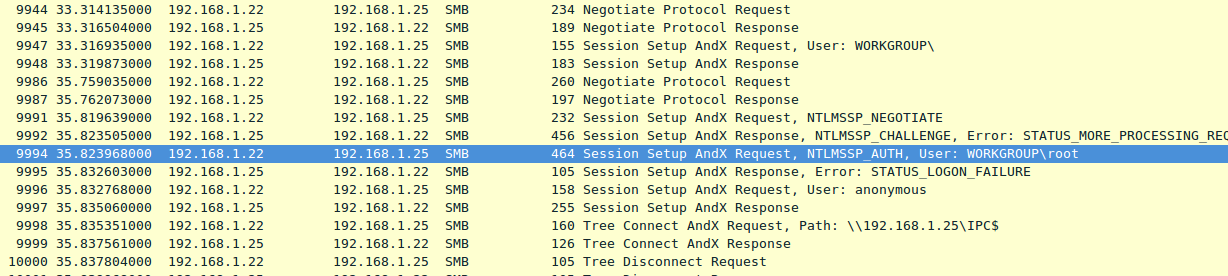
\includegraphics[width=\textwidth]{img/ws1.png}
    \caption{Tentative de connexion en \textit{root} sur la cible Windows}
    \label{fig:1}
\end{figure}
Comme nous pouvons le voir, la réponse du poste cible est négative (paquet 9995). Cette dernière précise \enquote{\textit{NT Status: STATUS\_LOGON\_FAILURE (0xc000006d)}}. L'accès en mode \enquote{credentials} n'a pas été configuré pour l'administrateur.\\
C'est pourquoi, lors de son deuxième essai, OpenVAS va tenter de se connecter grâce aux identifiants qui lui été fournis lors de la configuration de la cible. Ici, c'est avec l'utilisateur \enquote{\textit{bobby}} qu'il va le faire comme le montre la figure \ref{fig:2} (paquet 10166) :
\begin{figure}[H]
    \centering
    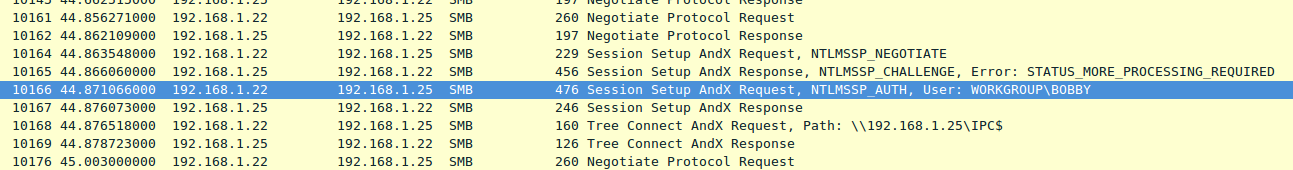
\includegraphics[width=\textwidth]{img/ws2.png}
    \caption{Tentative de connexion en temps que \enquote{\textit{bobby}} sur la cible Windows}
    \label{fig:2}
\end{figure}
Cette fois-ci, la connexion n'est pas un échec puisque le poste cible va alors répondre par \enquote{\textit{NT Status: STATUS\_SUCCESS (0x00000000)}} (paquet 10167). \\
Les échanges fait par les paquets 10168 et 10169 montrent qu'il a été possible d'accéder au registre de la cible.\\
Plus tard dans les échanges, nous pouvons constater qu'OpenVas a aussi accès aux disques partagés (ici C:), comme nous pouvons le voir sur la figure \ref{fig:3} (paquet 193383) :
\begin{figure}[H]
    \centering
    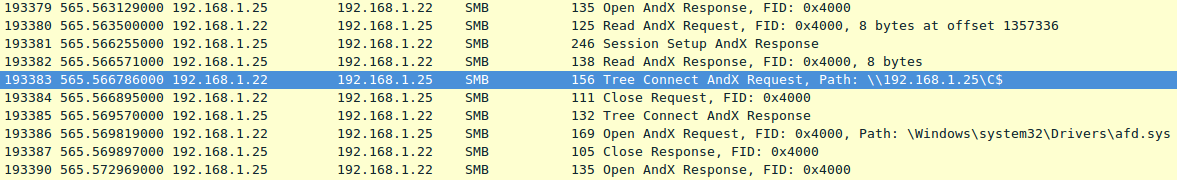
\includegraphics[width=\textwidth]{img/ws3.png}
    \caption{Accès aux disques partagés de la cible}
    \label{fig:3}
\end{figure}
Enfin, les échanges effectués par les paquets 326638 et 326639 nous prouvent qu'OpenVAS a aussi pu accéder aux données de l'administrateur. Nous pouvons voir cela sur la figure \ref{fig:5}.
\begin{figure}[H]
    \centering
    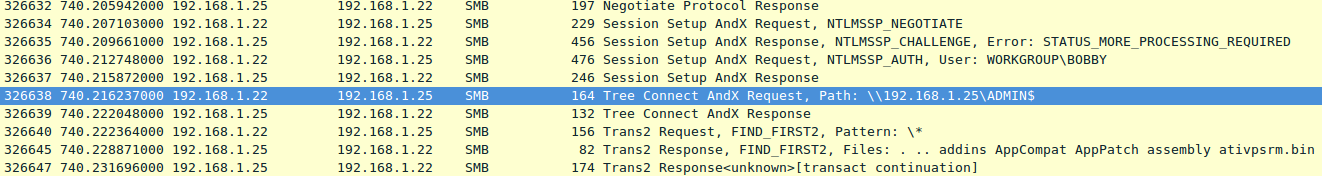
\includegraphics[width=\textwidth]{img/ws4.png}
    \caption{Accès aux données administrateur de la cible}
    \label{fig:5}
\end{figure}
\paragraph{Rapport de vulnérabilités}~\\\par
Une autre façon de vérifier si le scan s'est bien effectué en mode \enquote{credentials} est de lire le rapport fourni par OpenVAS directement. En effet, sur la seconde page de ce dernier, nous pouvons trouver la partie \textit{Host Authentications}. Comme le montre la figure \ref{fig:4}, nous pouvons voir que notre scan, OpenVAS a bien réussi à se connecter en temps que \textit{bobby} via le port 445 avec le protocole SMB sur notre cible (\textit{192.168.1.25 - blackyfox-1.home}).
\begin{figure}[H]
    \centering
    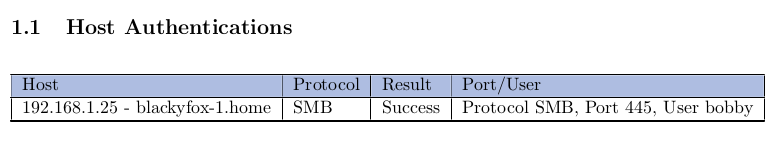
\includegraphics[width=\textwidth]{img/rep1.png}
    \caption{Résultat de l'authentification d'OpenVAS sur notre cible}
    \label{fig:4}
\end{figure}


\subsection{Cible sous Linux}
Pour le scan sous Linux, nous avons utilisé une version non mise à jour d'Ubuntu 14.10.\\
Après avoir créé un nouvel utilisateur en suivant la documentation fournie pour ce LAB, nous avions la configuration suivante sur la machine cible :
\begin{description}
 \item[Système d'exploitation :] Ubuntu 14.10
 \item[Nombre d'utilisateurs :] 3
 \item[Nom de l'utilisateur cible :] boby
 \item[Mot de passe du compte :] azerty
 \item[Adresse IP :] $192.168.1.10$
\end{description}

\newpage
% \rhead{2014-2015}
% \nocite{*}
\printbibliography\addcontentsline{toc}{section}{Références}
\newpage
\appendix
\section{Annexes}
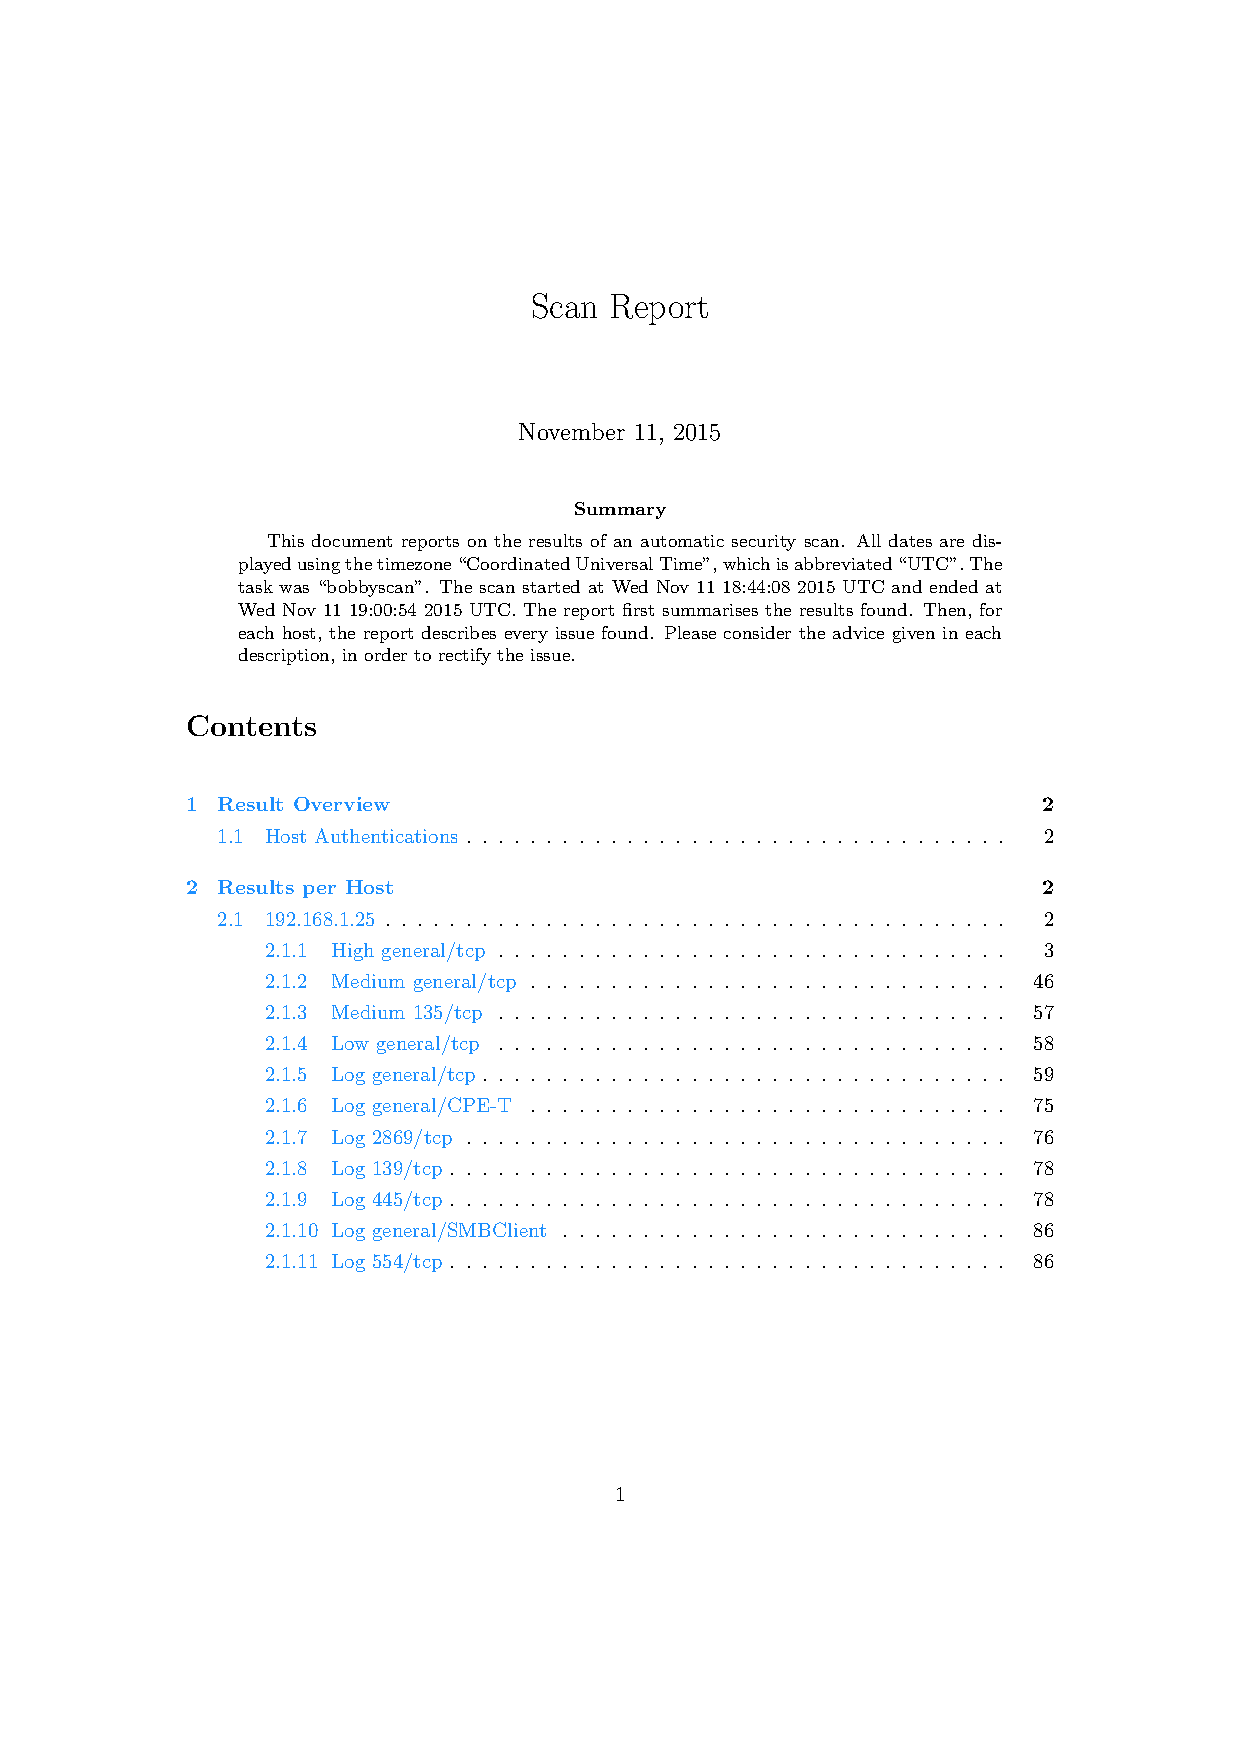
\includepdf[pages=1,scale=0.9,pagecommand=\subsection{Rapport de scan de vulnerabilite pour Windows 7 \label{VULNW7}}]{../Documents/win7.pdf}
\pagestyle{empty}
\includepdf[pages=2-,pagecommand={\thispagestyle{plain}}]{../Documents/win7.pdf}

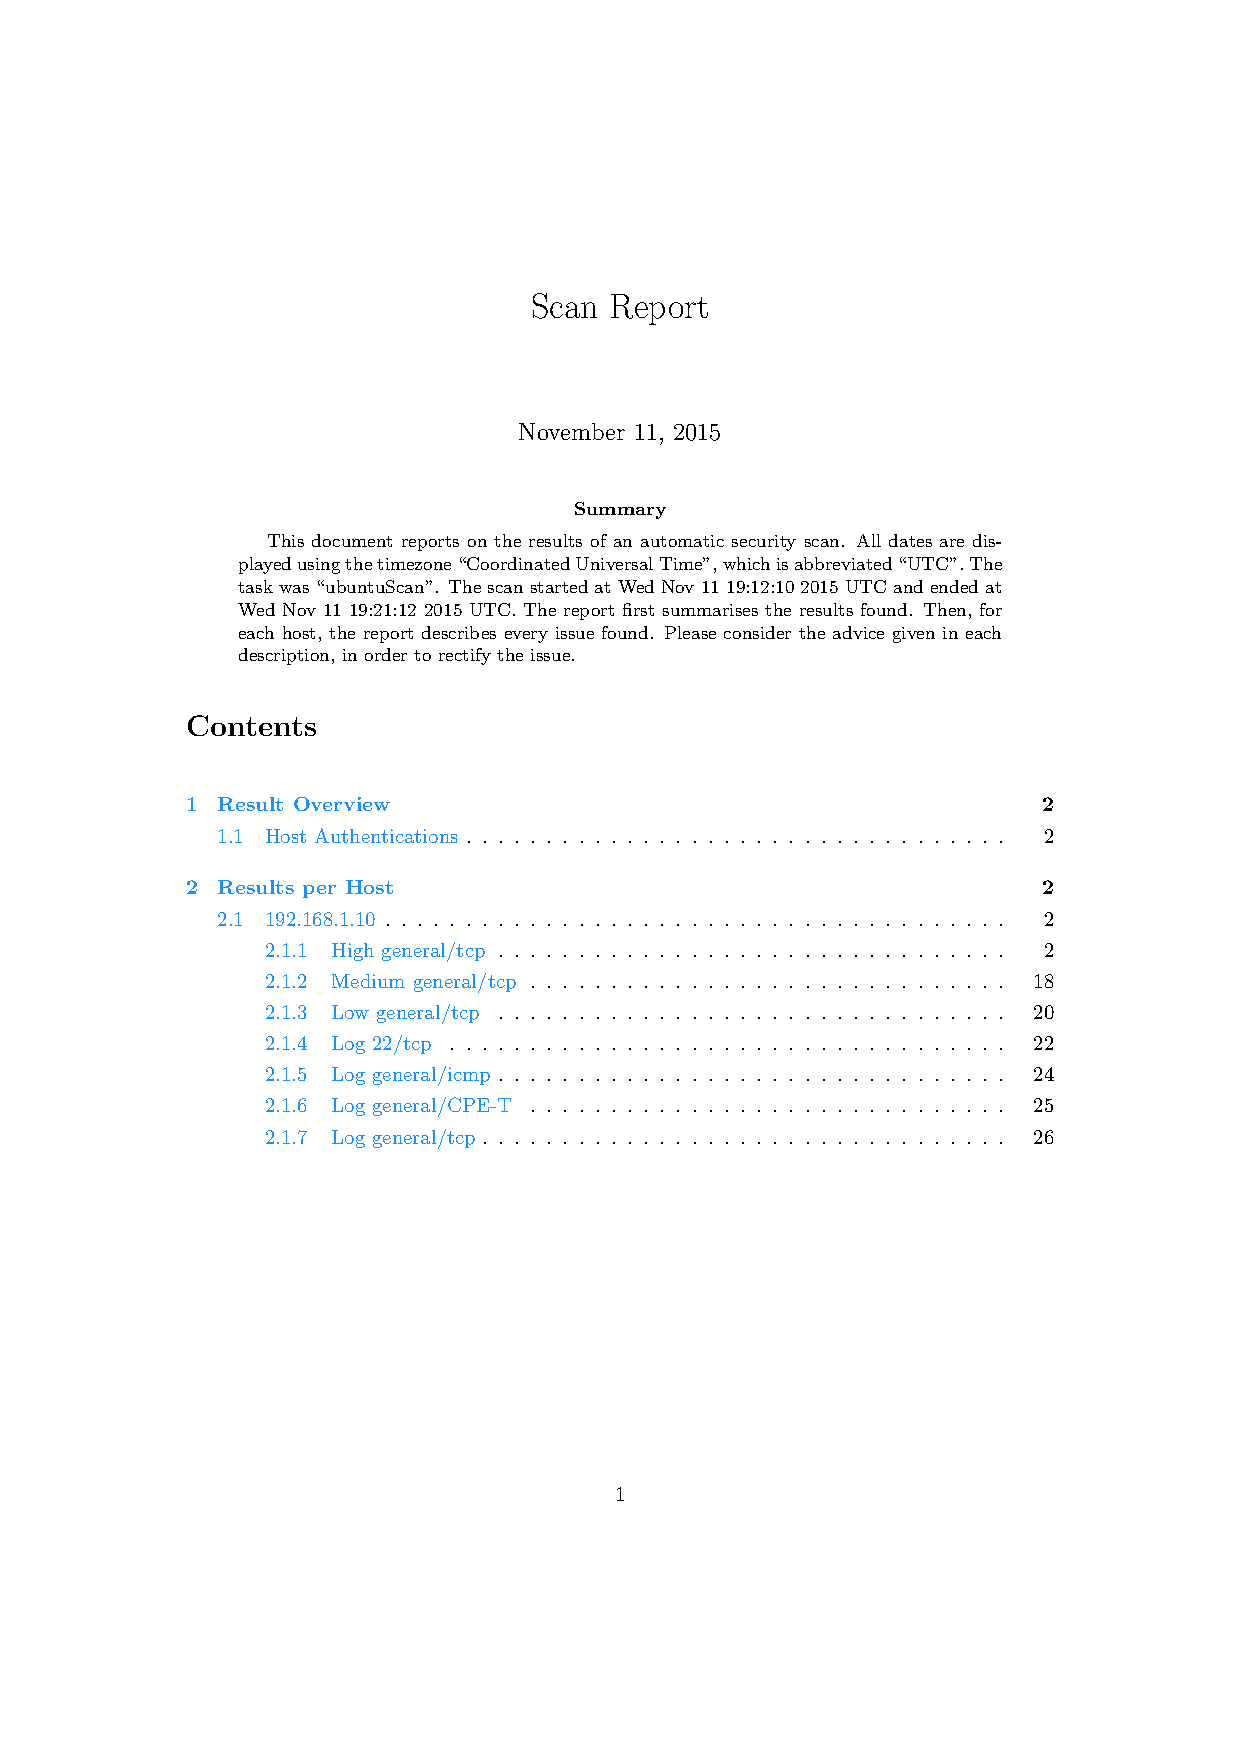
\includepdf[pages=1,scale=0.9,pagecommand=\subsection{Rapport de scan de vulnerabilite pour Ubuntu 14.10 \label{VULNU}}]{../Documents/ubuntu.pdf}
\pagestyle{empty}
\includepdf[pages=2-,pagecommand={\thispagestyle{plain}}]{../Documents/ubuntu.pdf}
% \glsaddall
% \printglossaries

%\listoffigures\addcontentsline{toc}{section}{\listfigurename}
\end{document}
\grid
